\documentclass[12pt]{article}

\usepackage{pablo}
\usepackage{pgfplots}
\usepackage{numprint}
\usepackage{multicol}
\usepackage[a4paper,margin=2cm]{geometry}
\usetikzlibrary{calc}

\pagestyle{empty}
\begin{document}

\begin{center}
  {\large
    Devoir surveillé --- 1h

    \textsc{Statistiques --- Vecteurs}
  }
\end{center}

\begin{exercice}[Vecteurs --- 8 points]
  $ABC$ est un triangle quelconque. Les points $D$, $E$, $F$, $G$, $H$ sont définis par :
  $\vecteur{AD}= \dfrac{5}{4}\vecteur{AB}$ ;
  $\vecteur{AE}= \dfrac{1}{4}\vecteur{AB}$ ;
  $\vecteur{AF}=-\dfrac{3}{4}\vecteur{AB}$ ;
  $\vecteur{AG}= \dfrac{1}{2}\vecteur{BA}$ ;
  $\vecteur{AH}= 2\vecteur{BC} - \dfrac{1}{2}\vecteur{AC}$.

  \begin{multicols}{2}
  \begin{center}
    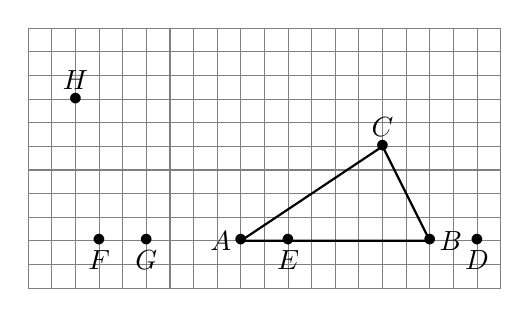
\begin{tikzpicture}[scale=0.3]
      \draw[thin,color=gray,step=1] (0,0) grid (20,11);
      \coordinate (A) at (9,2);
      \coordinate (B) at (17,2);
      \coordinate (C) at (15,6);
      \draw[thick] (A) -- (B) -- (C) -- cycle;
      \draw (A) node{$\bullet$} node[left]{$A$};
      \draw (B) node{$\bullet$} node[right]{$B$};
      \draw (C) node{$\bullet$} node[above]{$C$};

      \coordinate (D) at ($5/4*(B)-1/4*(A)$);
      \draw (D) node[below]{$D$} node{$\bullet$};

      \coordinate (E) at ($1/4*(B)+3/4*(A)$);
      \draw (E) node[below]{$E$} node{$\bullet$};

      \coordinate (F) at ($-3/4*(B)+7/4*(A)$);
      \draw (F) node[below]{$F$} node{$\bullet$};

      \coordinate (G) at ($3/2*(A)-1/2*(B)$);
      \draw (G) node[below]{$G$} node{$\bullet$};

      \coordinate (H) at ($(A)+2*(C)-2*(B)-1/2*(C)+1/2*(A)$);
      \draw (H) node[above]{$H$} node{$\bullet$};

    \end{tikzpicture}
  \end{center}

  \begin{enumerate}[(1)]
      \item \emph{Voir figure.}
      \item
      \begin{enumerate}[(a)]
        \item $\vecteur{ED}=\vecteur{EA}+\vecteur{AD}$\\
          $=-\frac{1}{4}\vecteur{AB}+\frac{5}{4}\vecteur{AB}$\\
          $=\frac{4}{4}\vecteur{AB}=\vecteur{AB}$
        \item $\vecteur{EF}=\vecteur{EA}+\vecteur{AF}$\\
          $=-\frac{1}{4}\vecteur{AB}-\frac{3}{4}\vecteur{AB}$\\
          $=-\vecteur{AB}$
        \item $\vecteur{ED}=\vecteur{AB}=\vecteur{FE}$, donc $E$ est le milieu de $[DF]$.
      \end{enumerate}
      \item
      \begin{enumerate}[(a)]
        \item $\vecteur{GH}=\vecteur{GA}+\vecteur{AH}$\\
          $=\dfrac{1}{2}\vecteur{AB}+2\vecteur{BC}-\frac{1}{2}\vecteur{AC}$
        \item $\vecteur{GH}=\dfrac{1}{2}\vecteur{AB}+2\vecteur{BC}-\frac{1}{2}\vecteur{AC}$\\
          $=\frac{1}{2}\vecteur{CB}+2\vecteur{BC}$\\
          $=\frac{3}{2}\vecteur{BC}$
        \item $\vecteur{GH}=\frac{3}{2}\vecteur{BC}$, donc les deux vecteurs sont colinéaires.
        \item Les vecteurs $\vecteur{GH}$ et $\vecteur{BC}$ sont colinéaires, donc les droites $(GH)$ et $(BC)$ sont parallèles.
      \end{enumerate}
  \end{enumerate}
\end{multicols}
\end{exercice}

\begin{exercice}[Statistiques : Définitions ; Effectifs et fréquences --- 4 points]
  Claude Got (chercheur en accidentologie) a étudié les accidents de la route
  mortels, en fonction du type d'usager.

  En 1960, sur les \numprint{8295} tués, \numprint{2540} étaient automobilistes, et \numprint{848} étaient
  cyclistes. Presque cinquante ans plus tard, en 2007, sur les \numprint{4620} tués, \numprint{2464}
    étaient automobilistes, et \numprint{142} étaient cyclistes.

  \begin{enumerate}[(1)]
    \item La population étudiée est les accidents de la route mortels (et non pas \emph{le nombre} d'accidents). Le caractère étudié est le type d'usagers. Ce caractère est qualitatif.
    \item En 1960, sur 8295 tués, 848 étaient cyclistes. Donc le pourcentage de cyclistes tués était $\frac{848\times100}{8295}=10\%$.
    \item En 2007, sur 4620 tués, 142 étaient cyclistes. Donc le pourcentage de cyclistes tués était $\frac{142\times100}{4620}=3\%$.
  \end{enumerate}
\end{exercice}

\begin{exercice}[Statistiques : Lecture graphique ; Médiane --- 8 points]
  \emph{Dans tout cet exercices, la lecture graphique étant approximative, j'ai considéré justes les réponses approchées.}
  \begin{center}
    \begin{tikzpicture}[scale=0.5]
      \begin{axis}[
          xscale=1.5,
          yscale=2,
          xmin=40,
          xmax=90,
          ymin=0,
          ymax=110,
          xlabel=Espérance de vie (années),
          y label style={below left},
          ylabel=Effectif (nombre de pays),
          grid=both,
          ybar interval,
          xminorgrids=false,
          xmajorgrids=false,
          ytick={0,10,...,110},
          minor ytick={0,5,...,110},
          extra y ticks={0,10,...,110},
          every extra y tick/.style={
            yticklabel pos=right,
          },
          minor grid style={gray},
          major grid style={black},
          xtick={40,50,...,90},% reset from ybar interval
          xticklabel={$[\pgfmathprintnumber\tick, \pgfmathprintnumber\nexttick[$}]],
        % a data file containing 8000 normally distributed
        % random numbers of mean 0 and variance 1
        \addplot+[hist={data=x,bins=5}] file {ds4-esperance.txt};
      \end{axis}
    \end{tikzpicture}
  \end{center}

  \begin{enumerate}[(1)]
    \item Par lecture graphique, on trouve que 43 pays ont une espérance de vie à la naissance comprise entre 60 et 70 ans.
    \item\label{moyenne} La moyenne est égale à :
      \[\frac{3\times45+27\times55+43\times65+100\times75+23\times85}{3+27+43+100+23}=70,77\]
    \item
      \begin{enumerate}[(a)]
        \item 
          \begin{tabular}{l|ccccc}
            Classes & $[40;50[$ & $[50;60[$ & $[60;70[$ & $[70;80[$ & $[80;90[$ \\
            \hline
            Effectifs & 3 & 27 & 43 & 100 & 23 \\
            \hline
            Eff. cumulés croissants & 3 & 30 & 73 & 173 & 196 \\
          \end{tabular}
        \item Il y a 196 valeurs, et $196\div2=98$, donc la médiane est la
          moyenne des 98 et 99\up{e} valeurs. Ces deux valeurs sont dans la
          classe $[70;80[$, donc cette classe est la classe médiane.
      \end{enumerate}
    \item
      \begin{enumerate}[(a)]
      \item L'espérance de vie à la naissance en France, 82 ans, est supérieure à la médiane. Par définition de la médiane, elle fait partie de la moitié des pays qui ont l'espérance de vie la plus haute.
      \item L'espérance de vie en Russie étant 70 ans, tous les pays des classes $[70;80[$ et $[80;90[$ ont des espérances de vie plus élevées. Cela représente $100+23=123$ pays, c'es-à-dire un pourcentage de $\frac{123\times100}{196}=62,76\%$.
    \end{enumerate}
  \item La moyenne calculée au \ref{moyenne} ne tient pas compte des tailles
    des pays : par exemple, si les pays très peuplés ont des espérances de vie
    faible, cela va faire baisser la moyenne.
  \end{enumerate}

\end{exercice}


\begin{exercice}[Bonus --- 2 points]
  Cent élèves participent à une épreuve notée sur 20 ; la moyenne de toutes les notes est 10.
  Les garçons sont 50\% de plus que les filles, et la moyenne des filles est 50\% de plus que celle des garçons.
  \begin{enumerate}[(1)]
    \item Soit $g$ le nombre de garçons, et $f$ le nombre de filles. Il y a 50\% de garçons de plus que les filles, donc $g=1,5f$. De plus, il y a 100 élèves, donc $g+f=100$. Ce qui donne :
      $1,5f+f=100$\\
      $2,5f=100$\\
      $f=100\div2,5=40$.

      Il y a donc 40 filles et 60 garçons.
    \item Soit $\bar f$ la moyenne des filles, et $\bar g$ celle des garçons. La moyenne de la classe, 10, est égale à :
      $\dfrac{40\bar{f}+60\bar{g}}{100}$. Or la moyenne des filles est 50\% plus élevée que celle des garçons, donc $\bar{f}=1,5\bar{g}$. Ainsi :\\
      $\dfrac{40\times1,5\bar{g}+60\bar{g}}{100}=10$\\
      $60\bar{g}+60\bar{g}=10\times100$\\
      $120\bar{g}=1000$\\
      $\bar{g}=1000\div120=8,33$.

      Donc la moyenne des garçons est 8,33, et celle des filles est $1,5\times8,33=12,5$.
  \end{enumerate}
\end{exercice}

\end{document}
